\section{What the network computes while it learns}\label{sec:trajectories}

Sections \ref{sec:networks}--\ref{sec:composition} concern \emph{whether} and \emph{when} the networks generalize. Here we ask \emph{what function} the network computes at each moment of training, and whether a general model reproduces the whole sequence of functions. Details are in \repo{study/trajectories/TRAJECTORIES.md}.

\paragraph{Setup.}
\begin{itemize}
\item \textbf{Targets.} Five chosen to differ in structure:
  \begin{itemize}
  \item sparsepoly $=\mathrm{sign}(2x_1+x_2x_3+x_4x_5x_6)$;
  \item a 5-term staircase;
  \item the multiplexer $x_4\,?\,x_1x_2x_3:\mathrm{MAJ}_3$;
  \item MAJ$(x_1x_2,x_3x_4,x_5x_6)$;
  \item MAJ of three MAJ$_3$.
  \end{itemize}
  Six held-out targets were run only after the models below were frozen.
\item \textbf{Conditions.} One-pass training, and fixed $n\in\{16384,2048,512\}$, with 3 seeds each.
\item \textbf{What is recorded.} At 72 log-spaced steps we record the network output on every pattern of the relevant variables $x_R$, each with 32 random settings of the irrelevant ones. This gives $f_R=E[f\mid x_R]$ exactly on the relevant cube, its full Fourier spectrum, and each target character's learned fraction $\varphi_S(t)=c_S(t)/\hat y_S$.
\end{itemize}

\begin{figure}[t]
\centering
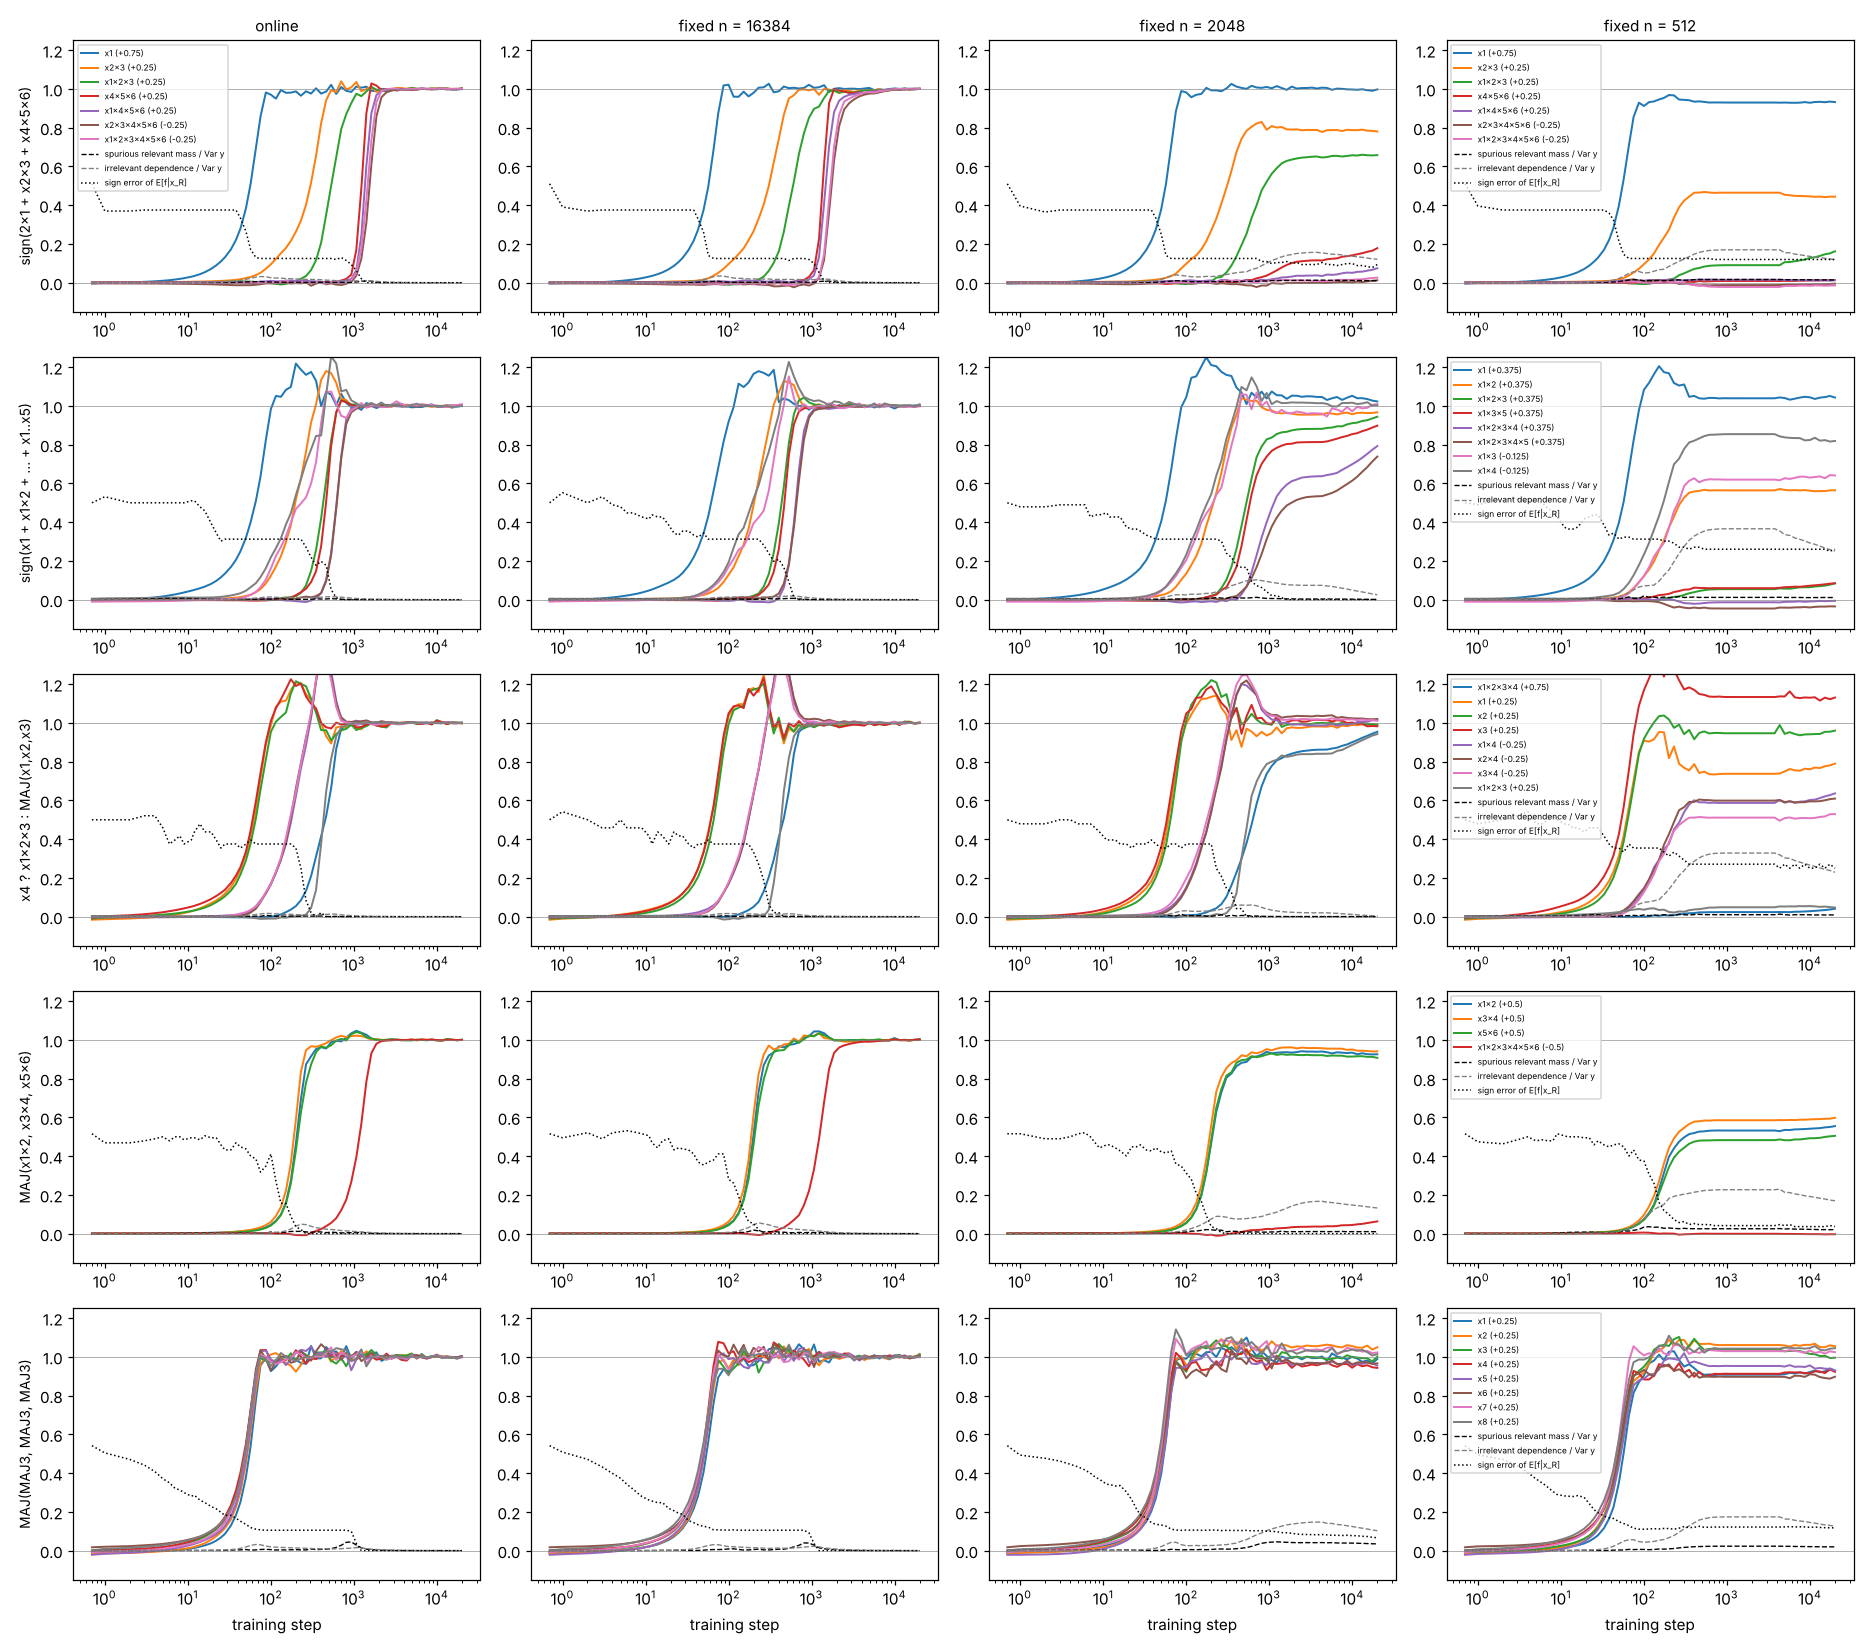
\includegraphics[width=\linewidth]{figures/trajectories.png}
\caption{Learned fraction of each Fourier character of the target (seed mean) against training step, for five targets (rows) and four conditions (columns). Dashed lines: spectral mass on characters the target does not have, and dependence on irrelevant inputs. Dotted line: sign error of $E[f\mid x_R]$.}
\label{fig:trajectories}
\end{figure}

\paragraph{The function on each plateau is a truncated Fourier expansion of the target} \status{Numerical}. On every plateau, $f_R$ is within 0.00–0.03 Var $y$ (at large $n$) of $P_{\mathcal S(t)}y=\sum_{S\in\mathcal S(t)}\hat y_S\chi_S$, the projection onto the characters learned so far.

The alternative ``the network fits everything about the inputs it has discovered'', $f_R\approx E[y\mid x_V]$, is 0.13–0.41 Var $y$ away on the same plateaus. For example, on MAJ$(x_1x_2,x_3x_4,x_5x_6)$ after the pairs, the distances are 0.003 against 0.225.

\paragraph{The sequence of functions} \status{Numerical} (\cref{fig:trajectories}).
\begin{itemize}
\item \textbf{Reproducibility.} The sequence is the same online and at $n=16384$, and seeds agree to about 15\% in onset step.
\item \textbf{The linear stage comes first,} at a nearly fixed 50–70 steps.
\item \textbf{Characters then arrive in bundles}, carried by one new feature direction:
  \begin{itemize}
  \item all $x_1x_j$ at once in the staircase;
  \item the three $x_ix_4$ in the multiplexer;
  \item about 500 characters of degree 2–8 in a 3-term DNF.
  \end{itemize}
\item \textbf{Order follows construction, not coefficient size.}
  \begin{itemize}
  \item The multiplexer's largest term, $x_1x_2x_3x_4$ (coefficient 0.75), comes last, after the features it is built from: steps 63, 172, then 437.
  \item In sparsepoly, $x_1$, $x_2x_3$, $x_1x_2x_3$ and $x_4x_5x_6$ (with its products) switch on at about 56, 297, 528 and 1389 steps.
  \end{itemize}
\item \textbf{Coefficients overshoot transiently,} by up to 1.36, as the readout refits on the features present.
\item \textbf{Finite $n$.} At finite $n$ the same sequence stops partway. Later stages saturate partially or never start, and memorization goes into the irrelevant inputs.
\end{itemize}

\paragraph{Three models} \status{Heuristic}. Each was calibrated on the five targets only, predicts $f_R(t)$ from the target alone, and was frozen (and committed) before any held-out network was run.
\begin{itemize}
\item \textbf{\texttt{fourier}, a by-hand rule.}
  \begin{itemize}
  \item \emph{Prediction.} $f_t=\sum_S\hat y_S\varphi_S(t)\chi_S$, with the fractions set by a race of \emph{moves}.
  \item \emph{Moves.} A move extends something already learned (nothing, a character, or a learned bundle) by $e$ new inputs at once. It learns every remaining character it reaches, as one bundle.
  \item \emph{Timing.} Duration $\propto\tau_0e^2\cdot2^{[\text{built on a feature}]}\cdot2^{[\text{odd degree}\ge3]}/\rho^{1/2}$, where $\rho$ is the bundle's share of the residual. A zero-bias ReLU gate has no first-layer gradient towards odd characters of degree at least 3.
  \item \emph{Finite $n$.} A memorization cut-off after a fixed number of epochs, and the spiked-estimation level $1-N/(n\rho^2)$.
  \end{itemize}
\item \textbf{\texttt{gates}.} A least-squares fit on greedily grown ReLU-gate bundles, with an alignment-law clock.
\item \textbf{\texttt{flow}.} The network's own Adam dynamics, reduced to the relevant inputs:
  \begin{itemize}
  \item the irrelevant inputs enter as Gaussian noise on each first-layer unit;
  \item the minibatch noise is kept in Adam's second moment;
  \item no constant is optimized against the networks.
  \end{itemize}
\end{itemize}

\begin{table}[t]
\centering\footnotesize\setlength{\tabcolsep}{4pt}
\begin{tabular}{lcccccc}
\toprule
& \multicolumn{3}{c}{calibration (5 targets)} & \multicolumn{3}{c}{held-out (6 targets)}\\
\cmidrule(lr){2-4}\cmidrule(lr){5-7}
traj against single seeds & online & $n=2048$ & $n=512$ & online & $n=2048$ & $n=512$\\
\midrule
\emph{network seed vs another seed} & \emph{0.0070} & \emph{0.0163} & \emph{0.0307} & \emph{0.0054} & \emph{0.0111} & \emph{0.0360}\\
\texttt{fourier} & 0.0087 & 0.0222 & 0.0188 & 0.0105 & 0.0177 & 0.0232\\
\texttt{gates} & 0.0096 & 0.0219 & 0.0196 & 0.0105 & 0.0205 & 0.0252\\
\texttt{flow} & 0.0042 & 0.0113 & 0.0208 & 0.0037 & 0.0097 & 0.0219\\
\bottomrule
\end{tabular}
\caption{Trajectory error, the mean over steps of $\lVert f_{\rm model}-f_{\rm net}\rVert^2/\mathrm{Var}\,y$, of each model against single network runs, next to one network run against another. A trivial step function (the target mean until step 1000, then the target) scores about 0.2.}
\label{tab:trajectories}
\end{table}

\paragraph{Results} \status{Numerical} (\cref{tab:trajectories}).
\begin{itemize}
\item \textbf{Out of sample.} All three models predict the held-out trajectories as well as the calibration ones.
\item \textbf{\texttt{flow}} predicts a network run better than an independent rerun of the network does, in every condition. Online, it puts held-out onsets within about 10\%.
\item \textbf{The two discrete rules} come within 1.3–2$\times$ of rerun-to-rerun variability at large $n$. \texttt{fourier}'s by-hand rule puts online onsets within about 25\%.
\item \textbf{Independent verification.} An agent per model regenerated every prediction bit for bit from the frozen commit, and found that no predictor reads any network data for the target it predicts. It also flagged two disclosures:
  \begin{itemize}
  \item the discrete rules have more tuned degrees of freedom than their five optimized constants: hand-tuned constants and structural switches chosen on calibration scores;
  \item the held-out targets, although new to this study, had been trained in the project's earlier fixed-$n$ study, whose data the models never read.
  \end{itemize}
\end{itemize}

\paragraph{Reading} \status{Heuristic}. The network computes a truncated Fourier expansion of the target and extends it in bundles. Each bundle is added by a move that builds on a feature it already has.
\begin{itemize}
\item \textbf{Cost.} A move is slower the more new inputs it must coordinate at once, and cheap when it composes existing features.
\item \textbf{Within a stage,} the readout refits on the features present.
\item \textbf{Finite $n$.} A race against memorization decides where the sequence stops.
\end{itemize}
This is the composition finding of \cref{sec:composition}, seen in time rather than in samples. The $e^2$ cost is a fixed-$d$ statement and does not include the $d^{k-1}$ dependence of \cref{sec:dscale}.
